\documentclass[12pt,letterpaper]{article}
\usepackage{natbib}

%Packages
\usepackage{xcolor}
\usepackage{color,soul}
\usepackage{pdflscape}
\usepackage{fixltx2e}
\usepackage{textcomp}
\usepackage{fullpage}
\usepackage{float}
\usepackage{latexsym}
\usepackage{url}
\usepackage{epsfig}
\usepackage{graphicx}
\usepackage{amssymb}
\usepackage{amsmath}
\usepackage{bm}
\usepackage{array}
\usepackage[version=3]{mhchem}
\usepackage{ifthen}
\usepackage{caption}
\usepackage{hyperref}
\usepackage{amsthm}
\usepackage{amstext}
\usepackage{enumerate}
\usepackage[osf]{mathpazo}
\usepackage{dcolumn}
\usepackage{lineno}
\usepackage{dcolumn}
\usepackage{hyphenat}
\usepackage[T1]{fontenc}
\usepackage{textcomp}
\newcolumntype{d}[1]{D{.}{.}{#1}}

\pagenumbering{arabic}


%Pagination style and stuff
\linespread{2}
\raggedright
\setlength{\parindent}{0.5in}
\setcounter{secnumdepth}{0} 
\renewcommand{\section}[1]{%
\bigskip
\begin{center}
\begin{Large}
\normalfont\scshape #1
\medskip
\end{Large}
\end{center}}
\renewcommand{\subsection}[1]{%
\bigskip
\begin{center}
\begin{large}
\normalfont\itshape #1
\end{large}
\end{center}}
\renewcommand{\subsubsection}[1]{%
\vspace{2ex}
\noindent
\textit{#1.}---}
\renewcommand{\tableofcontents}{}
%\bibpunct{(}{)}{;}{a}{}{,}

%---------------------------------------------
%
%       START
%
%---------------------------------------------

\begin{document}

%Running head
\begin{flushright}
Version dated: \today
\end{flushright}
\bigskip
\noindent RH: disparate views on disparity.

\bigskip
\medskip
\begin{center}

\noindent{\Large \bf Disparate views on disparity.} 
\bigskip

\noindent {\normalsize \sc Thomas Guillerme$^1$$^,$$^*$, Natalie Cooper$^2$, ..., Philip Donoghue$^3$}\\
\noindent {\small \it 
$^1$Imperial College London, Silwood Park Campus, Department of Life Sciences, Buckhurst Road, Ascot SL5 7PY, United Kingdom.\\}
\end{center}
\medskip
\noindent{*\bf Corresponding author.} \textit{guillert@tcd.ie}\\  
\vspace{1in}

%Line numbering
\modulolinenumbers[1]
\linenumbers

%---------------------------------------------
%
%       ABSTRACT
%
%---------------------------------------------

\newpage
\begin{abstract}

\begin{enumerate}
    blablalbalba
\end{enumerate}

\end{abstract}

\noindent (Keywords: disparity)\\

\vspace{1.5in}

\newpage 

%---------------------------------------------
%
%       INTRODUCTION
%
%---------------------------------------------

\section{Introduction}

\noindent \hl{\textit{1: disparity is observed everywhere}}
Biodiversity is not a smooth gradient of forms, functions, ecologies and behaviours but it is rather variable and discontinuous.
This is at the base of Biological Sciences and is linked to the concept of disparity with the observation that some groups of species are more similar or dissimilar than others.
This diversity in morphologies is in fact proper in nature and decoupled from taxonomic diversity: some groups may exhibit low diversity of species by high diversity of shapes \citep[or the other way around]{ruta2013,hopkinsdecoupling2013}.

\noindent \hl{\textit{2: historical evolution of disparity}}
Morphological diversity (hereafter disparity) is based on the observed the (dis)similarities between the morphologies of groups of organisms.
In palaeobiology, this concept, as a tool for macroevolutionary studies, stems from several seminal papers from the 90s describing and questioning how the diversity of life forms arose and evolved \citep{gould1989wonderful,gould1991disparity,briggs1992morphological,Wills1994,Foote01071994,Foote29111996,jernvall1996molar,foote1997evolution}.
In parallel, disparity analysis have been extended with modifications to macroevolutionary analysis based on continuous traits or geometric morphometric.
The former usage of data was popularised following \cite{Harmon961} and its implementation in \texttt{geiger} \citep{geiger2008}; while the latter was popularised following \citep{zelditch2012geometric} %Probably older
and implementations in \texttt{geomorph} (\citealt{adams2013geomorph, adams2017geometric} and precursory work from \citealt{claude2008morphometrics}).


\noindent \hl{\textit{3: the great popularity leads it to be used in many methods}}

\cite{prentice2011} define disparity as: ``a term widely (albeit not always consistently) used to describe the range of forms in a group of organisms, or the difference among different body plans''.
Disparity is really popular (Fig. \ref{Fig:GoogleOccurences}):

\begin{figure}[!htbp]
\centering
   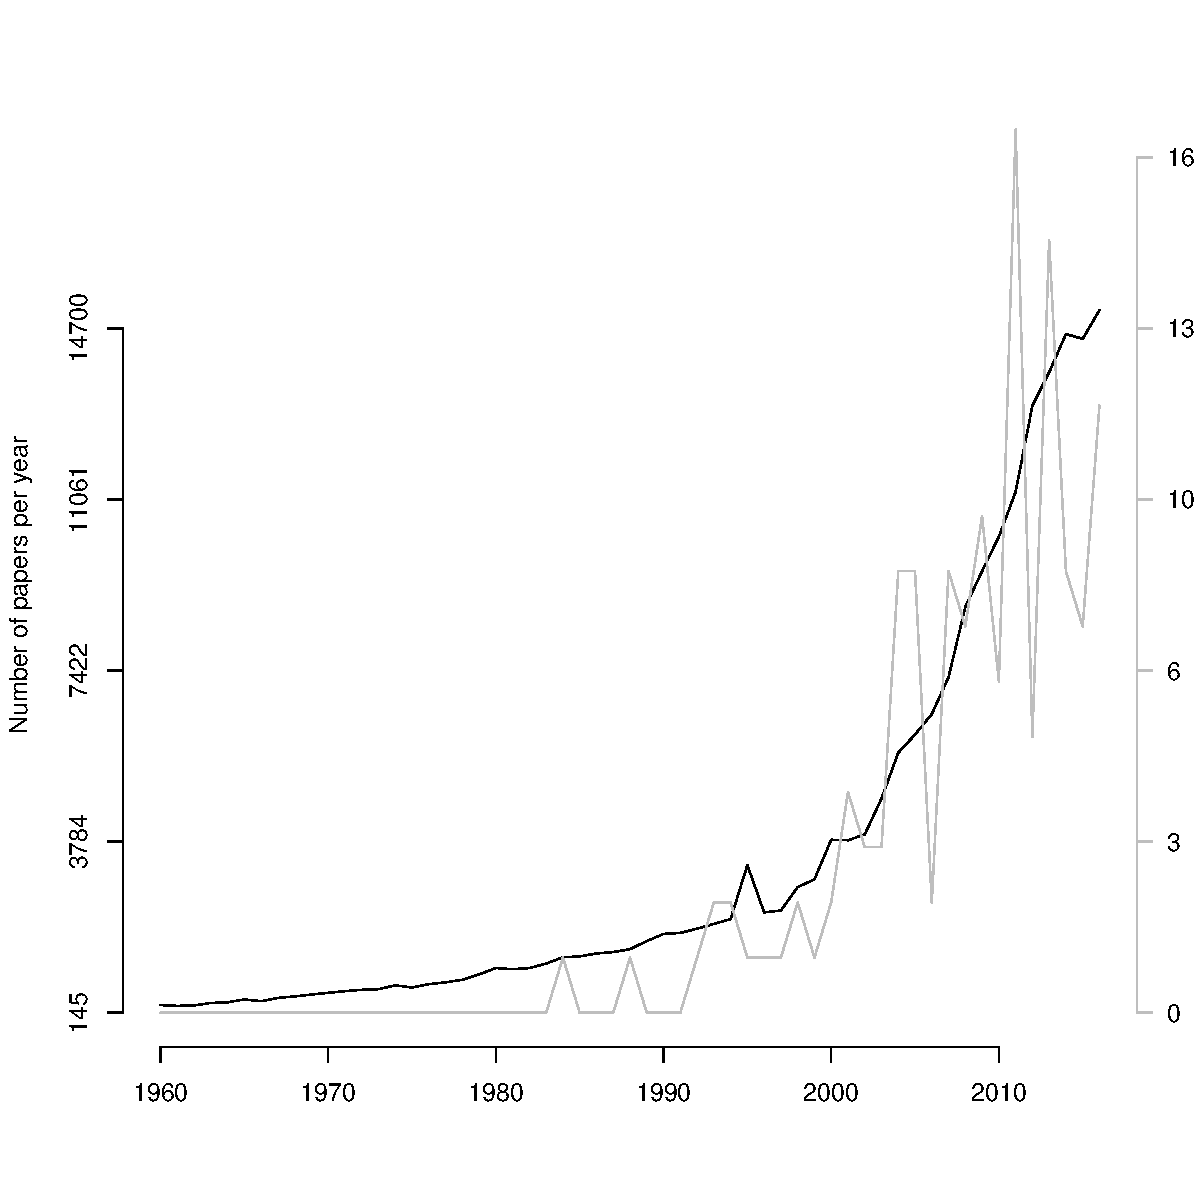
\includegraphics[width=1\textwidth]{Figures/GoogleScholarOccurences.pdf} 
\caption{Number of papers on Google Scholar matching the search ``morphological disparity'' per year. In black, the match is in the paper and in grey, in the title. We collected the number of matches per year from 1960 to 2016 in Google Scholar for the terms "morphological disparity" both in the text (fuzzy matching) or in the title (exact matching). The data was collected on the 1st of November 2017.}
\label{Fig:GoogleOccurences}
\end{figure}


\section{Why do we need disparity}

\noindent \hl{\textit{These points should be developed during the meeting}}


Which macroevolutionary questions are tackled through disparity analysis?
\begin{itemize}
    \item Bodyplan evolution through time
    \item Why does some morphologies exist and other not?
    \item tempo and mode of innovation of genuine novelty
    \item evolutionary competition
    \item effects of mass extinctions
    \item ecological niches
\end{itemize}

To answer these question, disparity has been used as a proxy for the biological increase/decrease of distinguishable morphological variation.
These proximal multidimensional spaces have been described as the morphospace, the eco-space, the functional space, the cladisto space, the developemental space, the allometric space, etc \citep[see][and references therein]{Hopkins2017}.
This multitude of multidimensional spaces arising from the observation of variable and discontinuous morphology in Life arises the question of their equivalence and their pertinence.
Are the description of these spaces all equivalent?
If disparity is the method or the metric describing these spaces then what \textit{is} disparity?

\section{What \textit{is} disparity (really)?}

Disparity can describe either the metric (disparity index \citep{Hopkins2017} or disparity metric \citep{Wills2001}) or the whole pipeline \citep{Claddis,zelditch2012geometric}

% §Methods for data:
\subsection{Data collection methodology}
To assess the usage of disparity in different published studies, we collected methodological data from the 500 first Google Scholar results for the key words ``morphological disparity'' per order of appearance (accessed on the 1st of November 2017).
For the 230 relevant papers among the 500 matches, we collected the following methodological data:

\begin{itemize}
    \item What was the focal biological group?
    \item What kind of data was measured (e.g. landmarks, discrete data, etc.)?
    \item Was data collected on the full organism or not?
    \item How was the morphospace explicitly defined (e.g. PCA, PCO, MDS, etc.)?
    \item How was the disparity metric(s) explicitly defined?
    \item Which statistical test was applied to test the disparity related hypothesis?
    \item Was phylogeny taken into account or not?
\end{itemize}

We used only the explicit definition of the morphospace and the disparity metric(s) in this search since a few number of papers had a vague definition of either or both (e.g. a disparity metric was measured but not described anywhere in the paper).

The remaining 270 matches were disparity was mentioned but not measured felt in the following categories: papers out of topic, papers mentioning morphological disparity without measuring it, review papers, papers not accessible (either through a broken link or a paywall) or referenced citation without the paper (as a Google Scholar match).

To reduce the amount of categories for the 230 recorded methods, we concatenated different methods in a smaller number of categories (see supplementary materials and \url{https://github.com/TGuillerme/Disparity_Working_Group/blob/master/Analysis/data_cleaning.Rmd}).

\begin{figure}[!htbp]
\centering
   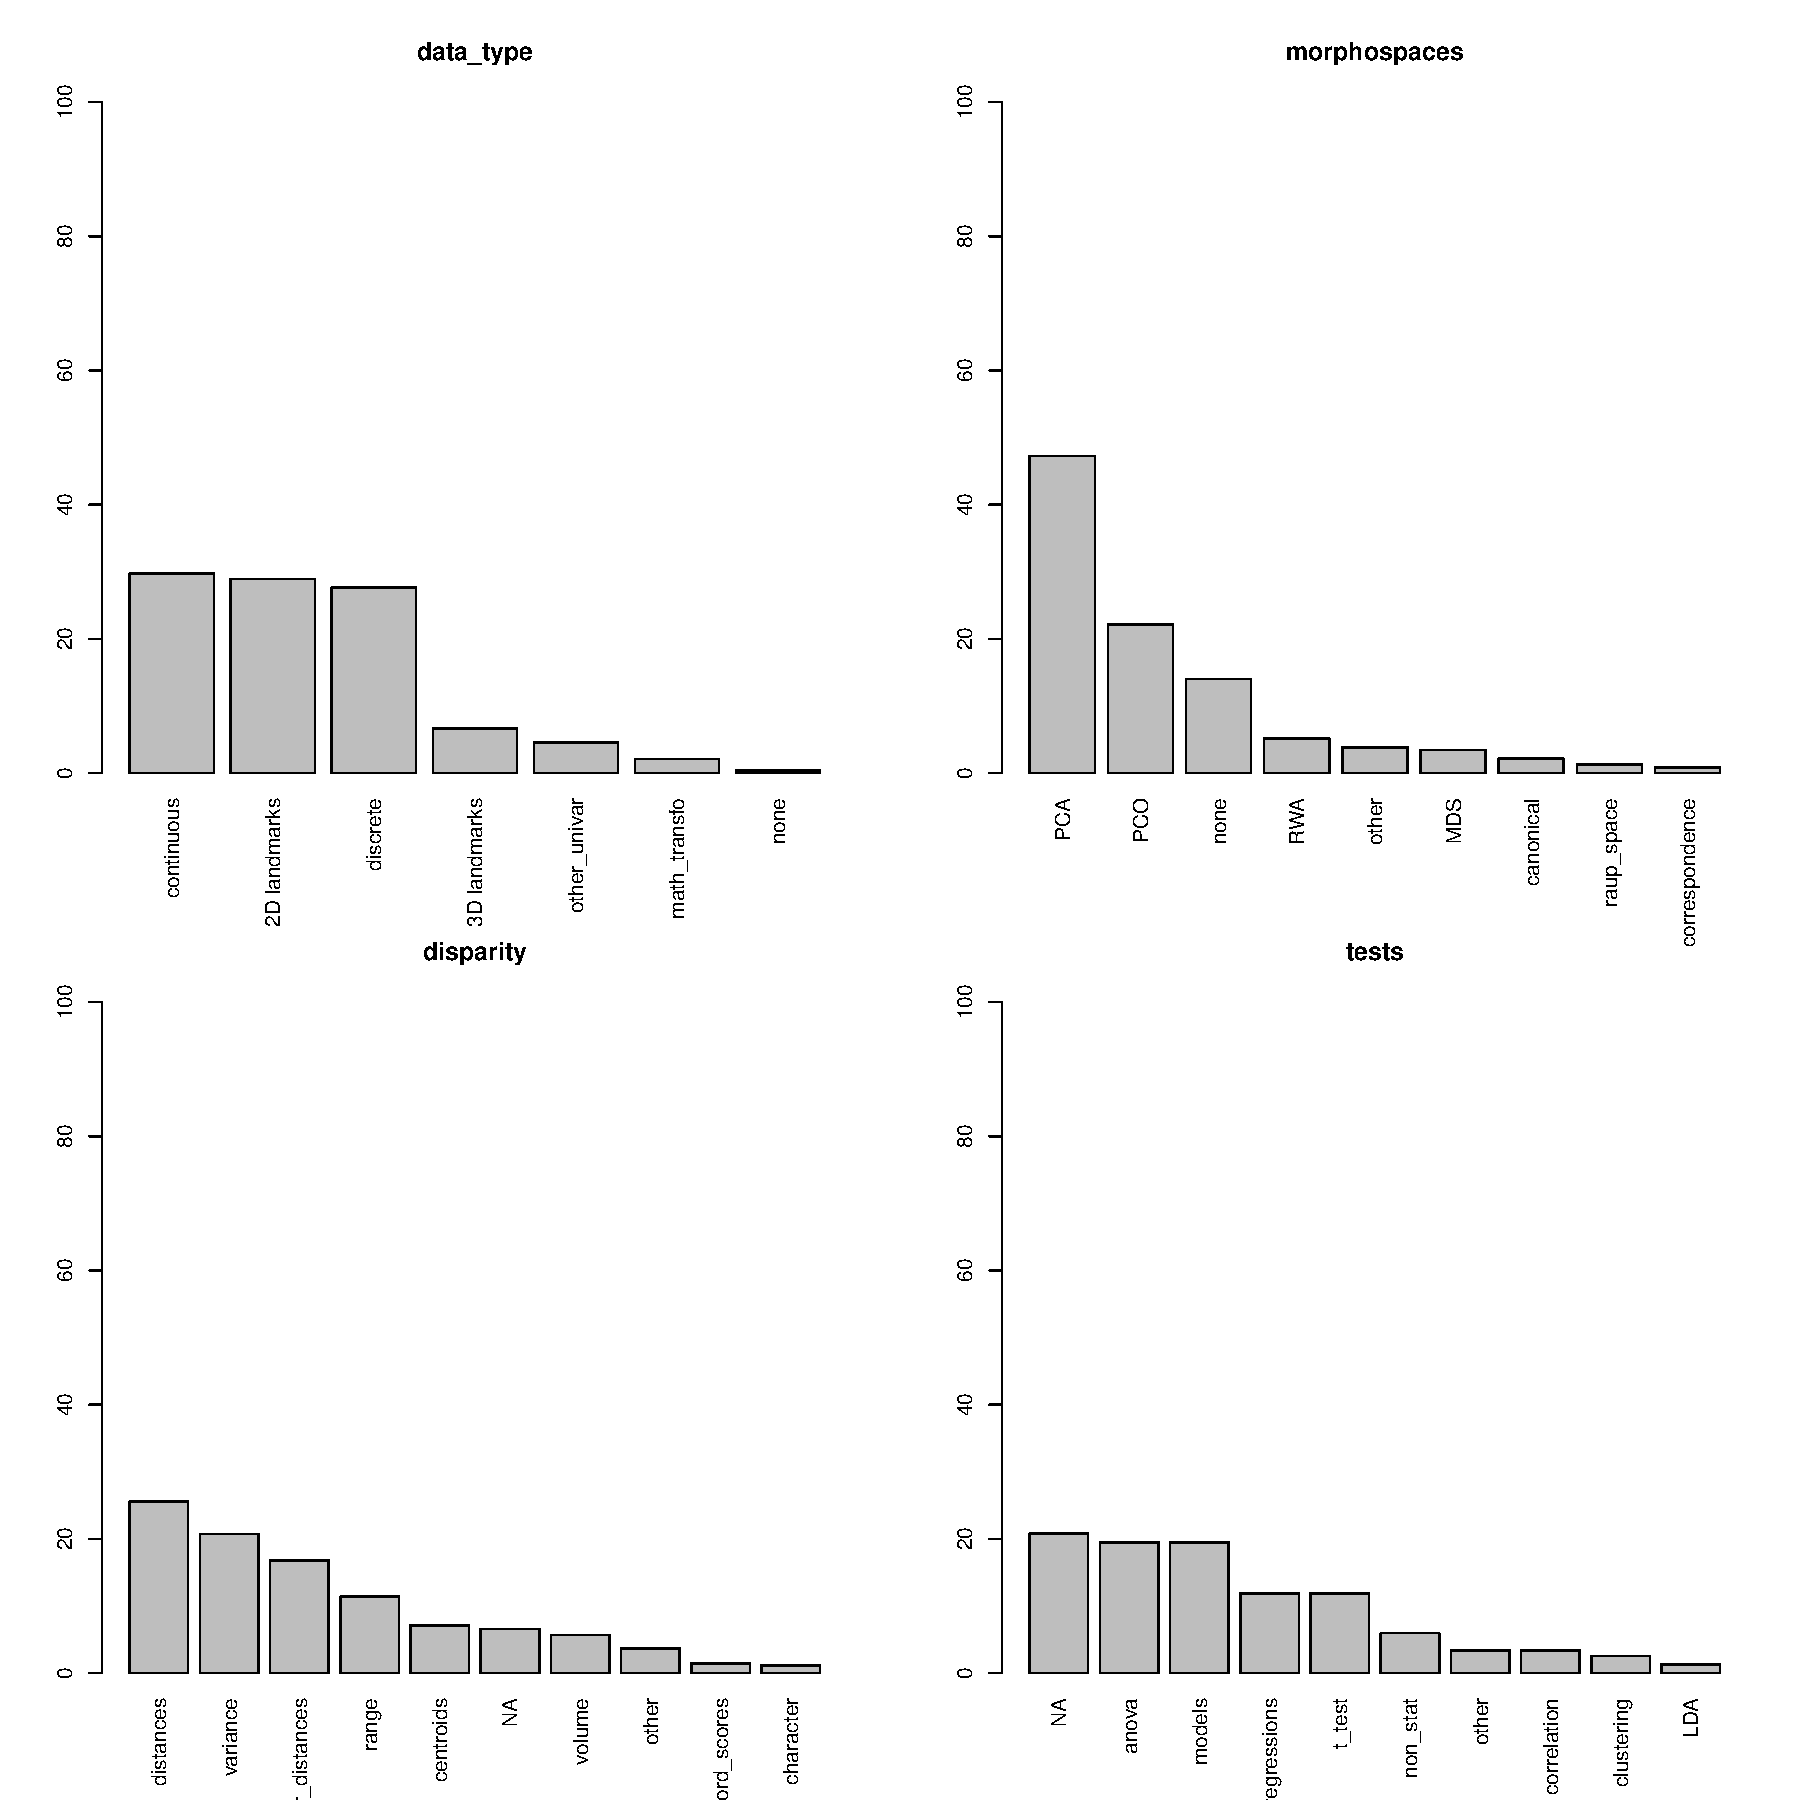
\includegraphics[width=1\textwidth]{Figures/MethodsProportions.pdf} 
\caption{Disparity methods proportional usage: (1) Data type: which input data was used (...); (2) Morphospace: how was the morphospace obtained (...); (3) disparity: what type of disparity metric was calculated (...); (4) test: what type of test was applied (...).}
\label{Fig:MethodsProportions}
\end{figure}

\hl{[ADD Biological group, full organism and phylogeny in the supplementary]}

\noindent \hl{\textit{These points should be developed during the meeting}}


\subsection{Disparity data}
The data used for disparity methods comes from three main sources:
\begin{itemize}
    \item Continuous data such as limb or body measurements \citep{slaterCetacean}.
    \item Discrete morphological characters \citep[sometimes referred to as ``Cladistic'' characters; ][]{Brusatte12092008}.
    \item Geometric morphometric data which is generally the Procrustes transformation of 2D or 3D landmarks \citep{cooney2017mega}.
\end{itemize}

However, data was by far not limited to these three categories (e.g. colours \citealt{maia2013key}; metabolic rate \citealt{nespolo2016studying} or chemicals signal \citealt{garcia2017heterogeneous}).

\subsection{Morphospaces}
\begin{itemize}
    \item PCAs [CITE].
    \item PCOs [CITE]
    \item Pairwise distance matrices \citep[no ordination; ][]{Harmon961}.
\end{itemize}

But also RWA [CITE] or Raup-spaces [CITE].

\subsection{Disparity metrics}
Throughout the 230 analysed papers, we found 103 unique combinations of metrics!

\begin{itemize}
    \item Distances measurements between species or from a certain point in the morphospace [CITE].
    \item Ranges and variances of each axis of the morphospace \cite{Wills2001,Ciampaglio2001}
    \item Distance between species based on the pairwise distance matrix (not the ordinations) [CITE].
\end{itemize}

But also metrics based on the volume [CITE], the characters dissimilarity [CITE] or the coordinates of some axis of the ordination [CITE]

\subsection{Disparity hypothesis}
Describing the many outputs (what and how is it tested):

\begin{itemize}
    \item Variance based (ANOVA, etc.) [CITE].
    \item Correlation based [CITE].
    \item Regression based (PGLS, etc.) [CITE].
\end{itemize}

But also discriminant analysis [CITE] and clustering [CITE].

\subsection{The three main disparity analysis}
From the collected data, we can highlight the use of three main different disparity analysis with their associated data/morphospace/metric/tests and related to specific methodological implementations.

\begin{itemize}
    \item \textbf{The ``\texttt{Claddis}'' approach:} this group of methods uses discrete morphological data (sometimes referred to as ``Cladistic'' characters) for the full organisms to build a PCO from the organism's pairwise distance as a morphospace. Disparity is then often measured as a variation of the ordinated matrix dimensions' variances or ranges (e.g. the sum of variance or/and the sum of ranges). Hypothesis are often tested using multivariate ANOVAs on the pairwise distance matrix or by simply comparing the confidence intervals overlap of the disparity from different groups. 

    \item \textbf{The ``\texttt{geomorph}'' approach:} this group of method is based on landmark data (2D or 3D) on parts of the organism studied usually the skull) and use a Procrustes transformation of the landmarks that are then directly ordinated using a PCA (but sometimes RWA). Disparity is often measured as a distance metric (e.g. the distance between the species and a point in the morphospace such as its centroid). Hypothesis are then tested using ANOVA type tests with usually no phylogenetic correction (although phylogeny is sometimes used to correct the morphospace).

    \item \textbf{The ``\texttt{dtt}'' approach:} this method can directly use continuous or discrete data for the full organism without any ordination (but not necessarily), and will measure disparity as the average pairwise distance between species (whether euclidean or any other type of distance). Hypothesis of higher/lower disparity can then be measured using null evolutionary models.

\end{itemize}

Of course some studies use a combination of these three methods or none of them at all!

Also, among each category XX\% of studies use multiple approaches.

[ADD Biological group, full organism and phylogeny in the supplementary]

\section{Expanding disparity}

How to compare disparity between groups? Is disparity relative?

How to compare disparity between methods?

Can we really say things about competition when looking at disparity in a single group?

Are all characters equal? Character contingency suggests otherwise

What is the relationship between disparity and tree shape?

Do we have a null model for investigating disparity?

Can we really say things about competition when looking at disparity in a single group?


\noindent \hl{\textit{Disparity in other fields}}

In ecology, disparity bears strong parallels with $\beta$-diversity in ecology (a measure of ecological communities (dis)similarity): one biological observation described by a vast array of metrics \citep{baselga2010partitioning, anderson2011navigating, donohue2016navigating}.

\section{Conclusion}

A quick guideline for good disparity analysis:

Maybe we need something like in Parham et al 2012 (Best Practices for Justifying Fossil Calibrations): an easy an identifiable description of the pipeline containing: 1) the type of data, 2) the morphospace and 3) the metric? 

\section{Acknowledgments}
The Royal Society.
TG acknowledge support from European Research Council under the European Union's Seventh Framework Programme (FP/2007 – 2013)/ERC Grant Agreement number 311092 awarded to Martin D. Brazeau.


\bibliographystyle{sysbio}
\bibliography{References}

\end{document}





% The multidimensional space can be defined in many ways and arise from many mathematical transformations of the data such as the pairwise distance matrix \citep{Close2015}, a principal coordinates analysis \citep[PCO;][]{Brusatte12092008}, a principal components analysis \citep[PCA;][]{zelditch2012geometric}, a multidimensional scaling \citep[MDS;][]{DonohueDim}, etc.
% Similarly, disparity metrics \citep[or indices;][]{Hopkins2017} can defined in many ways \citep[e.g.][or combinations thereof]{Wills2001,Ciampaglio2001,foth2012different,DonohueDim,Hughes20082013,finlay2015morphological,Close2015,diaz2016global}.
% Finally, difference between disparity metrics can also be measured in many ways: using NPMANOVA \citep[e.g.][]{Brusatte12092008}, multidimensional permutation test \citep[e.g.][]{diaz2016global} or even simple confidence interval overlap \citep[e.g.][]{halliday2016eutherian}.

% This variety of definitions and analysis have been developed in an equal variety of softwares such as \texttt{GINGKO} in javascript \citep{bouxin2005ginkgo,de2007ginkgo} or \texttt{geomorph} \citep{adams2013geomorph,adams2017geometric}, \texttt{Claddis} \citep{Claddis}, or \texttt{vegan} \citep{oksanen2007vegan} in R \citep{R}.
% This results in the need to learn different languages (or at least - when restricted to R - different packages with different standards) as well as making analysis sometimes idiosyncratic and often complex to repeat since they are based on a particular feature from a particular software.
% For example, in the excellent and widely used \texttt{geomorph} package morphological disparity analysis can be ran using the \texttt{morphol.disparity} function.
% Unfortunately, however, the multidimensional space can only be defined as the ordination of the procrustes transform of geometric morphometric landmarks, the disparity can only be defined as the Procrustes variance and the difference between groups can only be measured through permutation tests \citep{zelditch2012geometric,adams2013geomorph,adams2017geometric}.

% In all these analysis, each set of multivariate traits forms a multidimensional space.
% \hl{This space is represented as a matrix where rows are regarded as samples or observations (e.g. a specimen, field sites, etc.) and columns are variables or some transformation thereof (e.g. an embedding, scaling, ordination, etc. of the variables).}
% \hl{These multidimensional spaces can be defined in many ways, for example as a pairwise distance matrix (}
% \citealt{lloyd2016estimating}
% \hl{and references therein; e.g. in}
% \citealt{Close2015}
% \hl{), or as outputs from an ordination, whether it being a principal components analysis (PCA,}
% \citealt{PCA}
% \hl{; e.g. in}
% \citealt{zelditch2012geometric}
% \hl{), a metric scaling (PCO, PCoA,}
% \citealt{PCO}
% \hl{; e.g. in}
% \citealt{Brusatte12092008}
% \hl{) or a non-metric scaling (MDS, NMDS,}
% \citealt{MDS}
% \hl{; e.g. in}
% \citealt{Liow2004,DonohueDim}
% \hl{).}
% The name we give to the multidimensional space tends to vary with the kinds of traits used to construct it. 
% For example, when using morphological traits the multivariate space will be a morphospace, when using ecological traits it may be referred to as an ecospace or trait space.




% \hl{It is then possible to measure how the observations are distributed within this space to answer related questions (e.g. ``does group A occupies more space than group B?'').
% This requires the definition of a proxy for space occupancy: the disparity metric}
% \citep[or index;][]{Hopkins2017}
% \hl{which can be measured in a multitude of ways.}
% \hl{For example, one could use a metric based on the variance or the range of each axis of space}
% \citep{Wills2001, Ciampaglio2001}
% \hl{, a distance (e.g. Euclidean) measured between observations}
% \citep{foote1993contributions,Foote29111996}
% \hl{, a more direct approximation of the hyper volume }
% \citep{cornwell2006trait,DonohueDim}
% \hl{, or many more }
% \citep[e.g.][]{navarro2003MDA}.

% Finally, all these different multidimensional spaces and their associated disparity metrics can be used in an equal variety of statistical tests such as non-parametric multivariate analyses of variance (
% \hl{NPMANOVA, }
% \citealt{NPMANOVA}
% \hl{; e.g. in }
% \citealt{Brusatte12092008}
% \hl{)}
% multidimensional permutation tests
% \hl{(}
% \citealt{ManlyPermutations}
% \hl{; e.g. in }
% \citealt{diaz2016global}
% \hl{)}
% or even simply by looking at the confidence interval overlaps between disparity measurements
% \hl{().}
% In summary, there are many different ways to perform each step of a multidimensional analysis, making analyses of complexity ever more complex.

